%!TEX program = xelatex
\PassOptionsToPackage{full}{textcomp}
\documentclass[lang=en,11pt,a4paper,citestyle =authoryear,nobib=true]{elegantpaper}

% 标题
\title{HW3 - STAT 701}
\author{Wells Guan}

% 本文档命令
\usepackage{array,url,stix}
\usepackage{tikz}
\usepackage{tikz-cd}
\usepackage{enumitem}
\usepackage{amsmath}
\usepackage{amssymb}
\usepackage{listings}
\usepackage{subfigure}
\usepackage{placeins}

\lstset{
    frame=single,
    columns=fullflexible,
    keepspaces=true,
    showstringspaces=false,
    breaklines=true,
    breakatwhitespace=false,
    basicstyle=\ttfamily\footnotesize,
    numbers=left,
    numberstyle=\tiny,
    numbersep=6pt
}
\newcommand{\ccr}[1]{\makecell{{\color{#1}\rule{1cm}{1cm}}}}
\newcommand{\code}[1]{\lstinline{#1}}
\newcommand{\prvd}{$\hfill \qedsymbol$}
\newcommand{\Z}{\mathbb{Z}}
\newcommand{\R}{\mathbb{R}}
\newcommand{\N}{\mathbb{N}}
\newcommand{\C}{\mathbb{C}}
\newcommand{\Q}{\mathbb{Q}}
\newcommand{\M}{\mathcal{M}}
\newcommand{\B}{\mathcal{B}}
\newcommand{\X}{\mathcal{X}}
\newcommand{\Hil}{\mathcal{H}}
\newcommand{\range}{\mathcal{R}}
\newcommand{\nul}{\mathcal{N}}

% 文档区
\begin{document}
\maketitle

\noindent\textbf{Preface:} for all multitaper/DPSS related questions, you are welcome to use the R package \texttt{multitaper} (or python/Julia equivalents). You are also welcome to use chatbots or other external tools for hard Fourier integrals. It is not my intention for you to spend hours grinding out $\int_{-1/2}^{1/2}e^{i\omega h}e^{-\theta|\omega|}\,\mathrm d\omega$.

\subsection*{Problem 1}
Consider a sample path of length $n$ from a zero-mean, stationary time series $\{X_t\}_{t=1}^n$. Define its weighted Discrete Fourier Transform (DFT) at the Fourier frequencies $f_k=k/n$ for $k\in\{-[(n-1)/2],\ldots,[n/2]\}$, where $[\cdot]$ denotes the integer part of a number, by
\[
\widetilde X(f_k)=\sum_{t=1}^n w_tX_te^{-i2\pi f_kt}
\]
for a sequence of real-valued data taper weights $\{w_t\}_{t=1}^n$.
\begin{enumerate}[label=\arabic*.,leftmargin=*]
\item Let $w_t=n^{-1/2}$ for all $t$, so that $|\widetilde X(f_k)|^2=I(f_k)$ is the standard un-tapered periodogram estimator. Pick $n=512$ and a known autocovariance function $\gamma(h)$ for your process (e.g., an ARMA(p,q)). Using simulation:
\begin{enumerate}[label=(\alph*),leftmargin=*]
\item Draw $m\gg n$ independent sample paths (e.g., $m\approx10n$).
\item Compute the vector of DFT coefficients $\widetilde{\mathbf X}^{(i)}=[\widetilde X^{(i)}(f_k)]$ for Fourier frequency $f_k$ defined above for each realization $i=1,\ldots,m$.
\item Construct the empirical covariance matrix $\widehat\Sigma\in\mathbb C^{n\times n}=\sum_{i=1}^m\widetilde{\mathbf X}^{(i)}\widetilde{\mathbf X}^{(i)H}$ of these DFT coefficients.
\end{enumerate}
Inspect the matrix $\widehat\Sigma$ and comment on the resulting structure: how correlated are the estimates across different Fourier frequencies $f_k$ and $f_{k'}$? If you were interested to make a diagonal approximation of $\widehat\Sigma$, what information would you be throwing away?
\par\vspace{0.5em}\textbf{Sol.}\par

(a) The code for drawing (ARMA) sample paths:
\begin{lstlisting}[language=Python]
samples = np.stack([arma_generate_sample(
    ar=[1, -0.6],
    ma=[1, 0.3],
    nsample=N,
    scale=1,
    burnin=500,
    distrvs=rng.standard_normal,
    ) for i in range(M)])
\end{lstlisting}

(b) The code for computing DFT vectors for a single sample path:
\begin{lstlisting}[language=Python]
def simulated_paths(times_series, alpha = 10, rng=None):
    n = times_series.shape[0]
    weights = np.ones(n)/(n ** 0.5)
    frequencies = np.arange(-np.floor((n-1)/2),np.floor(n/2)+1)/n
    dft = np.stack([weighted_dft(times_series, weights, frequency) for frequency in frequencies])
    return dft

def weighted_dft(paths, weights, frequency):
    time = np.arange(1,paths.shape[0]+1)
    exp_term = np.exp( - 1j * 2 * np.pi * frequency * time)
    return np.sum(weights * paths * exp_term)
\end{lstlisting}

(c) The code of constructing:
\begin{lstlisting}[language=Python]
def empirical_dft_covariance(coefficients):
    dft_covaiance = np.outer(coefficients[0], coefficients[0].conj())
    for coefficient in coefficients[1:]:
        dft_covaiance += np.outer(coefficient, coefficient.conj())
    return dft_covaiance
\end{lstlisting}
and the structure of the matrix is shown the following:
\begin{figure}[htbp]
    \centering
    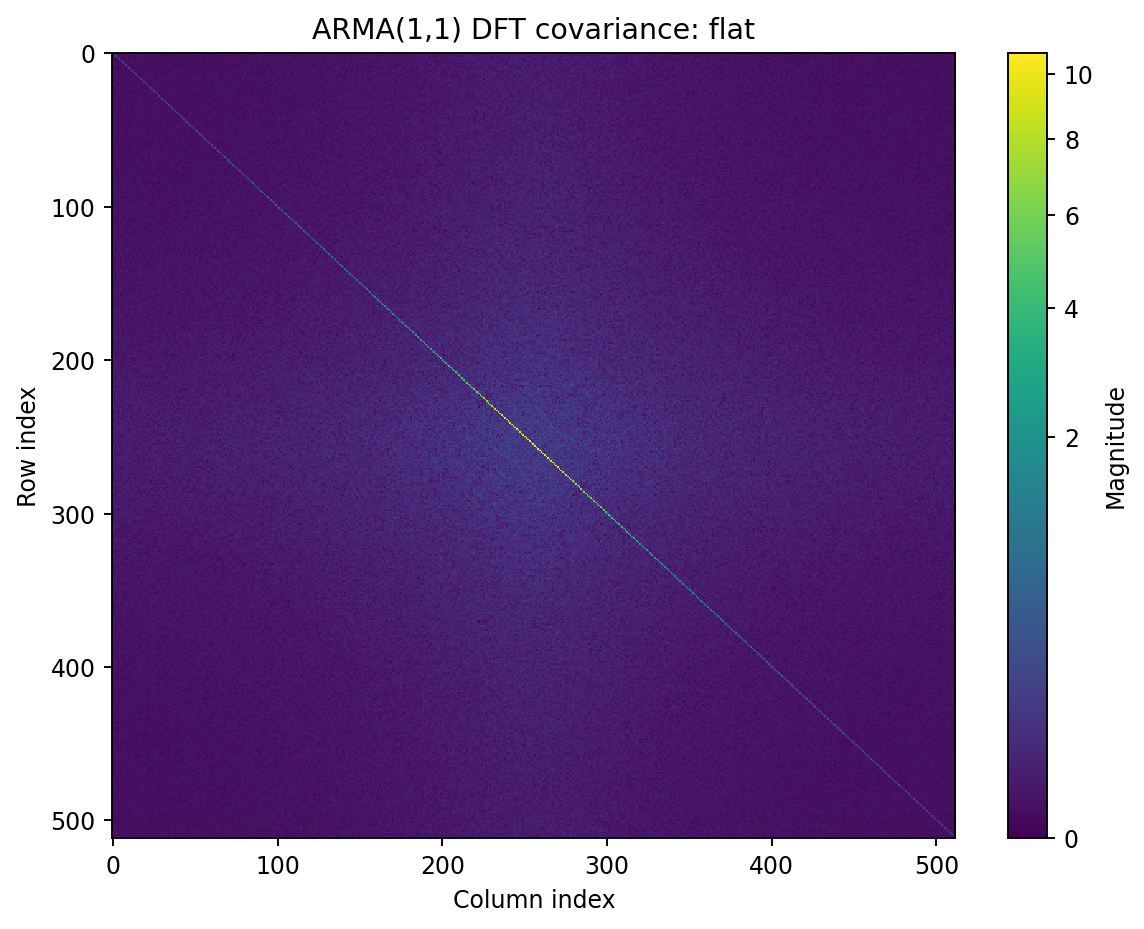
\includegraphics[width=0.85\linewidth]{png/empirical_covariance_matrix.png}
    \caption{Empirical covariance matrix of the DFT coefficients.}
    \label{fig:dft-covariance}
\end{figure}

I used the zero-mean Gaussian ARMA$(1,1)$ model
\[
X_t=0.6X_{t-1}+Z_t+0.3Z_{t-1},\qquad Z_t\sim N(0,1).
\]
Its known autocovariance is $\gamma(0)=2.265625$ and
$\gamma(h)=1.659375(0.6)^{|h|-1}$ for $|h|\geq1$.
I generated $m=5120$ independent paths of length $n=512$, discarding 500
initial observations. The code above returns the sum in the question;
for the figures I divide by $m$ to estimate the population covariance.
This rescaling does not change its structure.

The matrix is approximately diagonal, with the largest diagonal variances
near frequency zero. Large covariance magnitude does not by itself mean
large correlation. To separate these effects, I also use
\[
\widehat R_{k\ell}=\frac{\widehat\Sigma_{k\ell}}
{\sqrt{\widehat\Sigma_{kk}\widehat\Sigma_{\ell\ell}}}.
\]
For this model the mean magnitude of the theoretical adjacent-frequency
correlations is $0.00606$, compared with $0.01469$ in the simulation.
Some empirical off-diagonal values are Monte Carlo error: they need not
vanish in a finite sample of 5120 paths. A diagonal approximation retains
frequency-specific variances and discards all cross-frequency covariances,
including finite-window boundary effects. For the exact covariance its
relative Frobenius approximation error is $0.04367$; thus the error is small
in this example, rather than evidence of strong coupling to zero frequency.
Because the data are real, opposite-frequency DFT coefficients are complex
conjugates. A diagonal Hermitian covariance alone does not imply independence
of the entire two-sided complex DFT vector.


\vspace{2em}

\item Repeat this exercise using a normalized Slepian/discrete prolate spheroidal sequence (DPSS) taper sequence $w_t=h_t^{(0)}$ with time-bandwidth parameter $NW=10$. What structural differences do you observe in the empirical covariance matrix compared to the un-tapered case?
\par\vspace{0.5em}\textbf{Sol.}\par

I repeat the experiment with the same ARMA coefficients and the same
5120 sample paths, changing only the taper. The weights are obtained by
\begin{lstlisting}[language=Python]
weights = dpss(N, NW=10, Kmax=1, norm=2)[0]
\end{lstlisting}
so that $\sum_t w_t^2=1$. The wider band around the diagonal represents
strong correlations between nearby Fourier coefficients.

\begin{figure}[htbp]
    \centering
    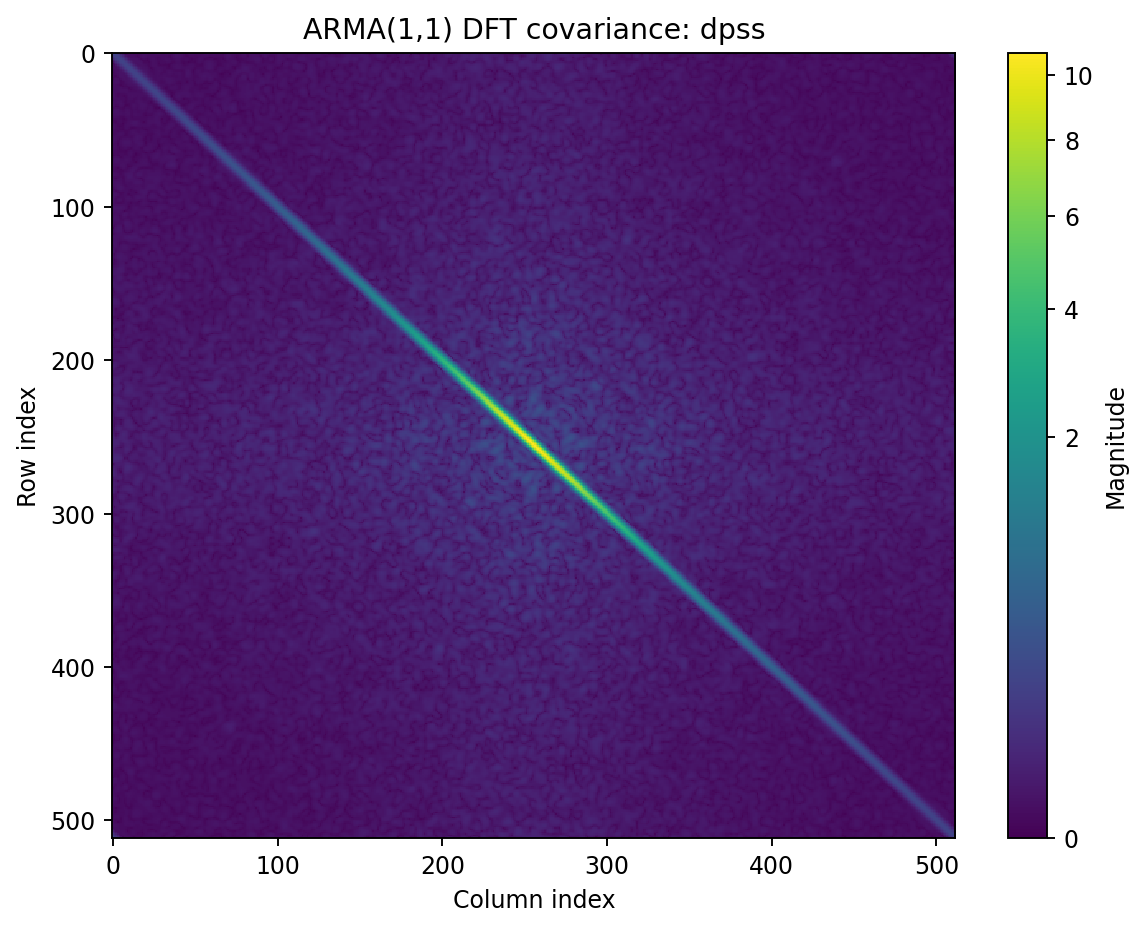
\includegraphics[width=0.85\linewidth]{png/empirical_covariance_matrix_dpss.png}
    \caption{Empirical covariance matrix of the DFT coefficients with DPSS weights.}
    \label{fig:dft-covariance-dpss}
\end{figure}

For a white-noise input with variance $\sigma^2$, the tapered covariance is
\[
\operatorname{Cov}(\widetilde X(f_k),\widetilde X(f_\ell))
=\sigma^2\sum_{t=1}^n w_t^2e^{-2\pi i(f_k-f_\ell)t}.
\]
Flat weights make this zero at distinct Fourier frequencies, but DPSS weights
do not. The taper improves spectral concentration while sacrificing the
orthogonality of adjacent weighted Fourier coefficients. In this ARMA
experiment, the mean theoretical adjacent correlation magnitude is $0.92436$
(empirical $0.92435$), and the relative Frobenius error of a diagonal
approximation is $0.88070$. The normalized correlation plot makes the band
visible away from the high-power central region as well.
\begin{figure}[htbp]
\centering
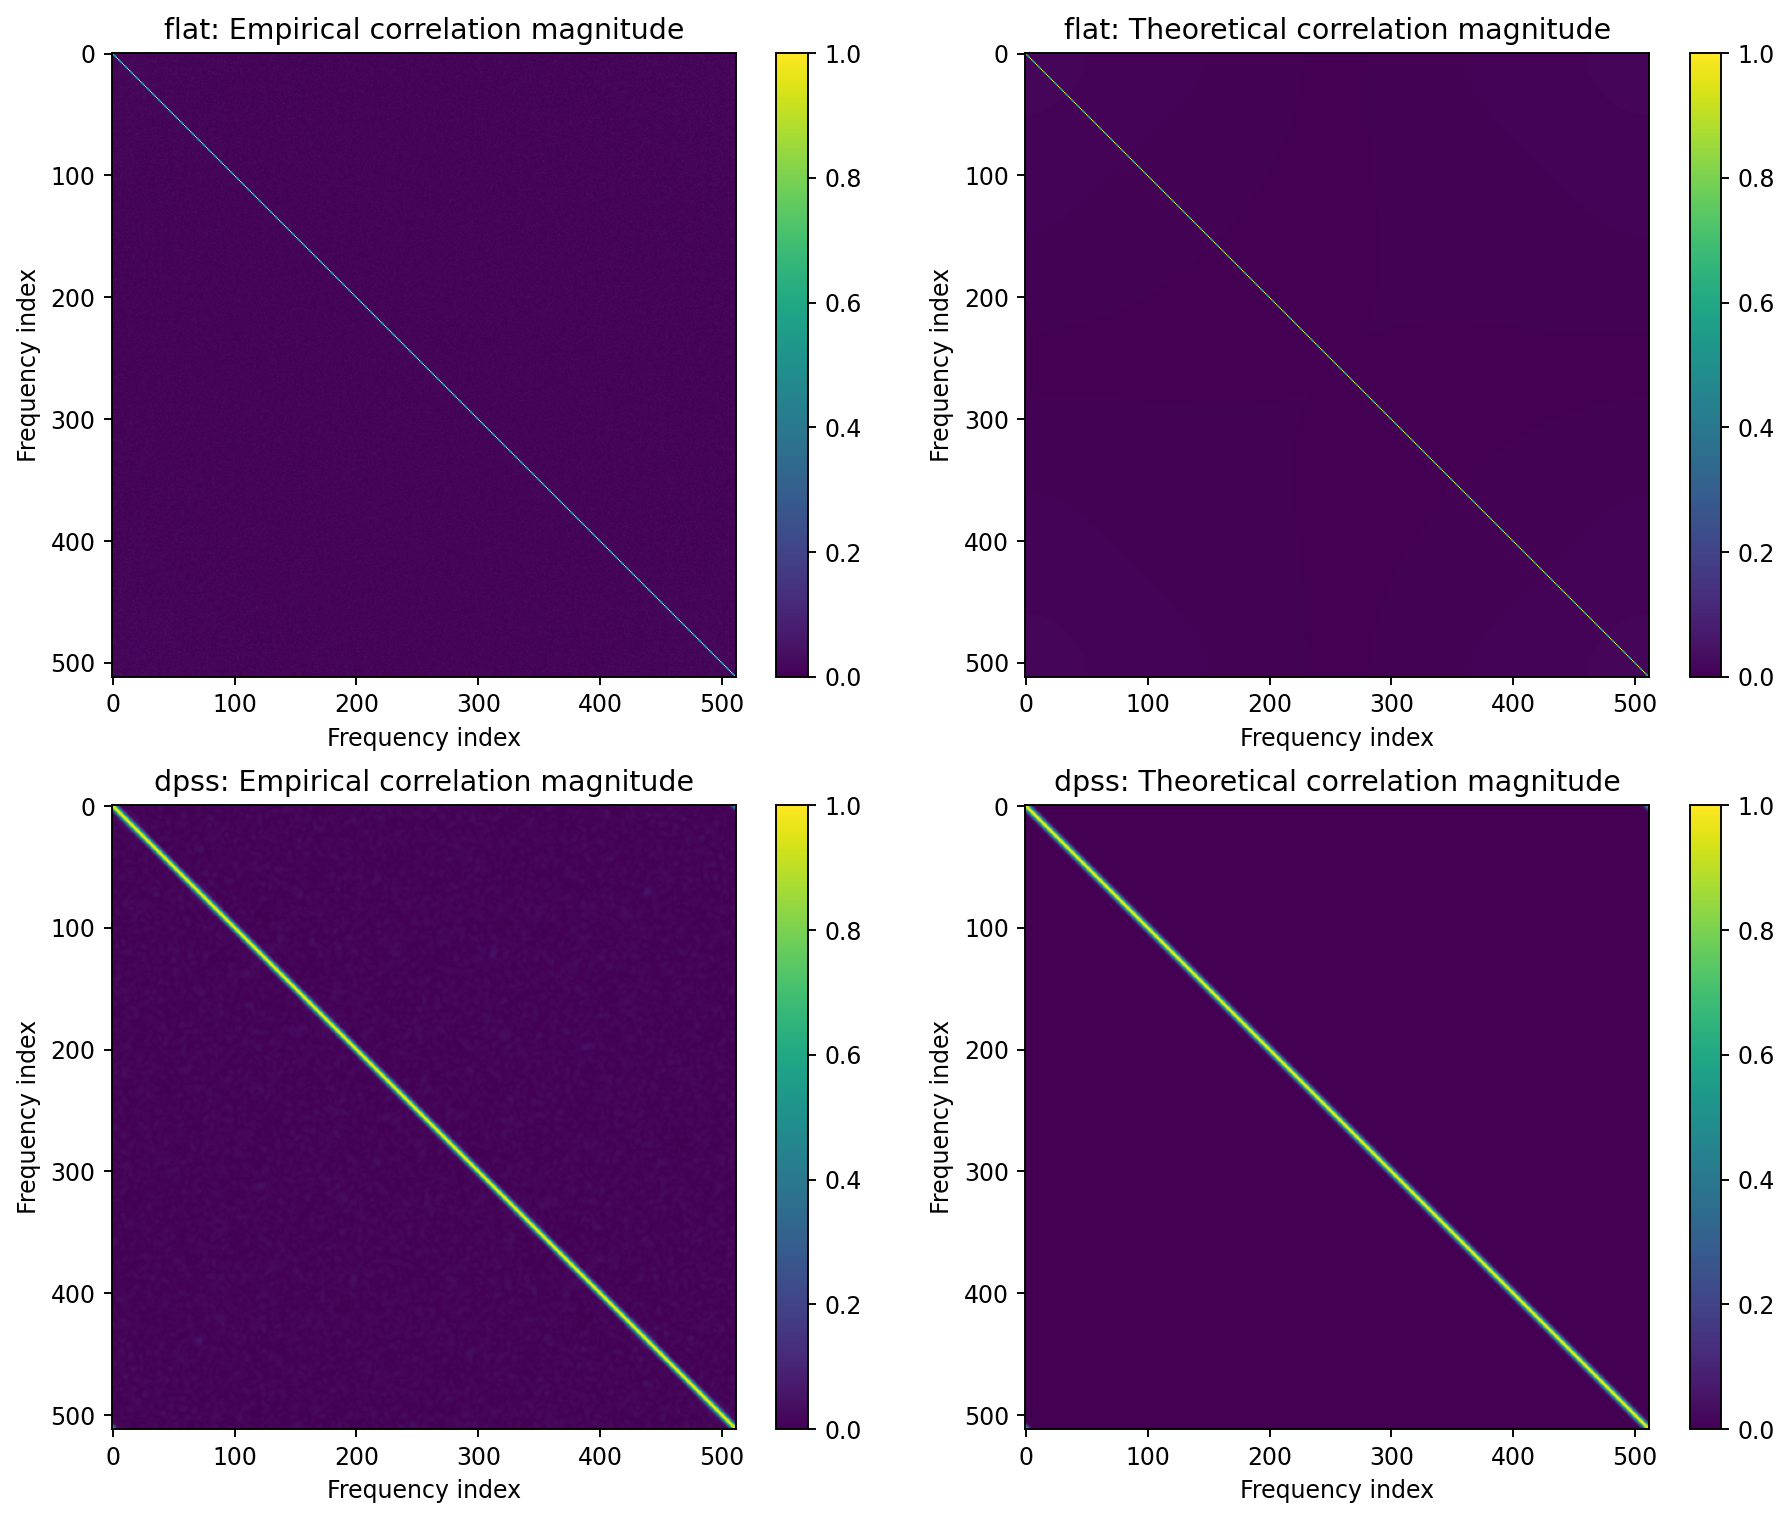
\includegraphics[width=0.96\linewidth]{png/problem1_correlation_comparison.png}
\caption{Empirical and exact correlation magnitudes for the same ARMA process.
All panels use the same linear color scale from zero to one.}
\label{fig:correlation-comparison}
\end{figure}

\vspace{2em}


\item[$3^*$.] Analytically derive the cross-covariance $\operatorname{Cov}(\widetilde X(f_k),\widetilde X(f_{k'}))$ for the flat weight sequence $w_t=n^{-1/2}$ in terms of the process spectral density $S(f)$ or autocovariance $\gamma(h)$. Simplify as much as possible using Dirichlet kernel properties. Based on your result, at what rate do you think these covariances go to zero?
\par\vspace{0.5em}\textbf{Sol.}\par

I use the complex covariance convention
$\operatorname{Cov}(U,V)=\mathbb E[U\overline V]$ for centered variables,
and frequencies in cycles per observation, so
$\gamma(h)=\int_{-1/2}^{1/2}S(f)e^{2\pi ifh}\,df$.
For $D_n(u)=\sum_{t=1}^ne^{-2\pi iut}$,
\[
D_n(u)=e^{-\pi i(n+1)u}\frac{\sin(\pi nu)}{\sin(\pi u)},
\]
with its continuous extension at integers. Expanding the covariance gives
\begin{align*}
C_{k\ell}
&=\frac1n\sum_{t,s=1}^n\gamma(t-s)e^{-2\pi i(f_kt-f_\ell s)}\\
&=\frac1n\int_{-1/2}^{1/2}
S(f)D_n(f_k-f)\overline{D_n(f_\ell-f)}\,df\\
&=\frac1n\sum_{|h|<n}\gamma(h)e^{-2\pi if_kh}
\sum_{s=\max(1,1-h)}^{\min(n,n-h)}e^{-2\pi i(f_k-f_\ell)s}.
\end{align*}
For $k=\ell$, the inner sum is $n-|h|$, giving the Fejer-smoothed spectrum
\[
C_{kk}=\sum_{|h|<n}\left(1-\frac{|h|}{n}\right)\gamma(h)e^{-2\pi if_kh}.
\]
For distinct Fourier frequencies modulo one,
$\sum_{s=1}^ne^{-2\pi i(f_k-f_\ell)s}=0$.
The shortened sum omits only $|h|$ terms, so
\[
|C_{k\ell}|\leq\frac1n\sum_{|h|<n}|h|\,|\gamma(h)|.
\]
Consequently, if $\sum_h|h|\,|\gamma(h)|<\infty$, as for our causal ARMA
model, the off-diagonal covariances are uniformly $O(n^{-1})$.
Absolute summability of $\gamma$ alone implies $o(1)$ by dominated
convergence, but need not give this rate. Stationarity alone does not imply
vanishing cross-frequency covariance or a universal rate.
For white noise the off-diagonal covariances are exactly zero.
\vspace{1em}
\end{enumerate}

\FloatBarrier
\subsection*{Problem 2}
Let's explore the local versus broadband bias tradeoffs in spectral density estimation.
\begin{enumerate}[label=\arabic*.,leftmargin=*]
\item Write code that uses circulant embedding to \emph{exactly} simulate a length-$n$ sample path from a stationary time series with arbitrary covariance function $\gamma(\cdot)$. Please design its interface to accept an ACF sequence $\{\gamma(0),\ldots,\gamma(n-1)\}$ and return the length-$n$ sequence. You may use a built-in library for the FFT, but please do the other book-keeping yourself.
\par\vspace{0.5em}\textbf{Sol.}\par

The code uses the symmetric circulant first row
\[
c=(\gamma(0),\ldots,\gamma(n-1),\gamma(n-2),\ldots,\gamma(1)),
\qquad L=2(n-1).
\]
Its eigenvalues are $\lambda=\operatorname{FFT}(c)$. With a real vector
$z\sim N(0,I_L)$, I compute
\[
y=\operatorname{IFFT}\bigl(\sqrt\lambda\,
\operatorname{FFT}(z)\bigr).
\]
The FFT and IFFT normalizations cancel to give
$\operatorname{Cov}(y)=F^*\operatorname{diag}(\lambda)F/L$,
the circulant covariance with first row $c$. Its first $n$ coordinates
therefore have exactly the required Toeplitz covariance, without burn-in.
Here is the main implementation:
\begin{lstlisting}[language=Python]
row = np.r_[acf, acf[-2:0:-1]]
eigenvalues = np.fft.fft(row).real
white_noise = rng.standard_normal(len(row))
sample = np.fft.ifft(
    np.sqrt(eigenvalues) * np.fft.fft(white_noise)
).real
return sample[:len(acf)]
\end{lstlisting}
This construction requires nonnegative circulant eigenvalues. An arbitrary
valid Toeplitz covariance does not guarantee that this particular embedding
is positive semidefinite. The full code checks this condition, clips only
roundoff-sized negative eigenvalues, and otherwise raises an error rather
than silently changing the covariance. A longer valid covariance extension
or another exact Gaussian method would then be needed. All embeddings used
below passed the check. As a numerical validation, 20,000 independent draws
with $n=8$ and $\gamma(h)=0.7^{|h|}$ gave a maximum covariance-entry error
of $0.0251$ against the exact Toeplitz matrix.
\vspace{1em}

\item Recall the periodogram and the multitaper estimator described in class. Please design spectral densities/covariance functions to achieve the following failure modes, and demonstrate them by simulating data and computing the estimators:
\begin{enumerate}[label=(\alph*),leftmargin=*]
\item The multitaper estimator misses two distinct peaks and only reports one, but the periodogram gets them both.
\par\vspace{0.5em}\textbf{Sol.}\par

I use $n=4096$ and
\[
\gamma(h)=0.994^{|h|}\{
\cos(2\pi\,0.160h)+\cos(2\pi\,0.164h)\}
+0.05\,1_{\{h=0\}}.
\]
For each component, the corresponding spectrum is the sum of two shifted
Poisson kernels:
\[
S_j(f)=\frac12\sum_{\epsilon\in\{-1,1\}}
\frac{1-r^2}{1+r^2-2r\cos(2\pi(f-\epsilon f_j))},\qquad r=0.994.
\]
The peaks are separated by $0.004$, exceeding the Fourier grid spacing
$1/4096$, but smaller than the multitaper smoothing width
$2W=2(24)/4096=0.01171875$. I compute the periodogram and average 47
unit-norm DPSS estimates with $NW=24$:
\begin{lstlisting}[language=Python]
tapers = dpss(n, NW=24, Kmax=47, norm=2)
f, raw = periodogram(sample)
f, mt = multitaper_spectrum(sample, tapers)
\end{lstlisting}
The periodogram resolves the two clusters near the true peaks. The multitaper
estimate averages across both peaks and produces one broad feature. This is
local smoothing bias, not a failure of the simulation.
\begin{figure}[htbp]
\centering
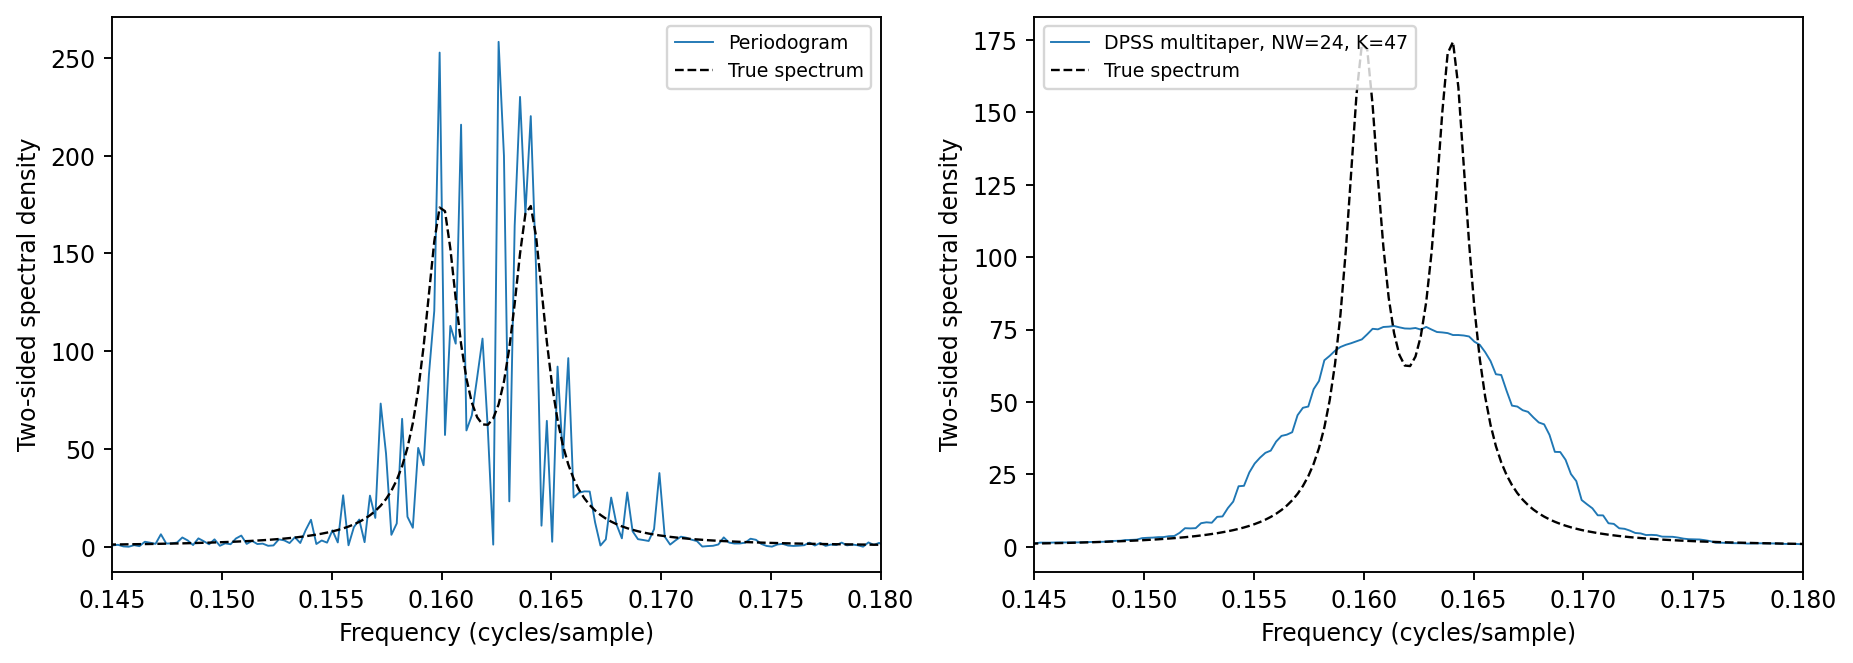
\includegraphics[width=0.98\linewidth]{png/problem2_resolution.png}
\caption{The same realization analyzed with the periodogram and a wide-band
DPSS multitaper. Dashed curves are the true spectrum.}
\label{fig:resolution}
\end{figure}
\vspace{1em}
\item The periodogram loses a faint spectral peak, but the multitaper catches it.
\par\vspace{0.5em}\textbf{Sol.}\par

I construct a broad but faint peak on a white-noise floor, together with a
strong peak elsewhere. Define the periodized Gaussian peak
\[
G_{v,c,b}(f)=\frac{v}{2\sqrt{2\pi}b}
\sum_{j\in\mathbb Z}\left[
 e^{-(f-c+j)^2/(2b^2)}+e^{-(f+c+j)^2/(2b^2)}\right].
\]
Its autocovariance is $v e^{-2\pi^2b^2h^2}\cos(2\pi ch)$. I use
\[
S(f)=1+G_{2,0.10,0.004}(f)+G_{0.02,0.27,0.006}(f),
\qquad n=4096.
\]
The peak at $0.27$ rises only from a background near 1 to approximately
$1.665$. The unaveraged periodogram fluctuates enough that it is difficult
to distinguish this broad feature from unrelated spikes. With $NW=8$ and
15 DPSS tapers, the variance is reduced and the weak elevated band becomes
visible. The half-bandwidth $8/4096$ is small relative to the weak peak's
width, so smoothing is useful here rather than merging distinct features.

For 128 additional independent simulations, at the grid point nearest
$0.27$, the periodogram had mean $1.8439$ and standard deviation $1.5298$;
the multitaper had mean $1.5616$ and standard deviation $0.4146$.
These are Monte Carlo summaries, not exact expectations. The multitaper
reduces noise substantially at the price of modest downward peak bias.
Neither estimator is guaranteed to detect a weak peak in every realization.
\begin{figure}[htbp]
\centering
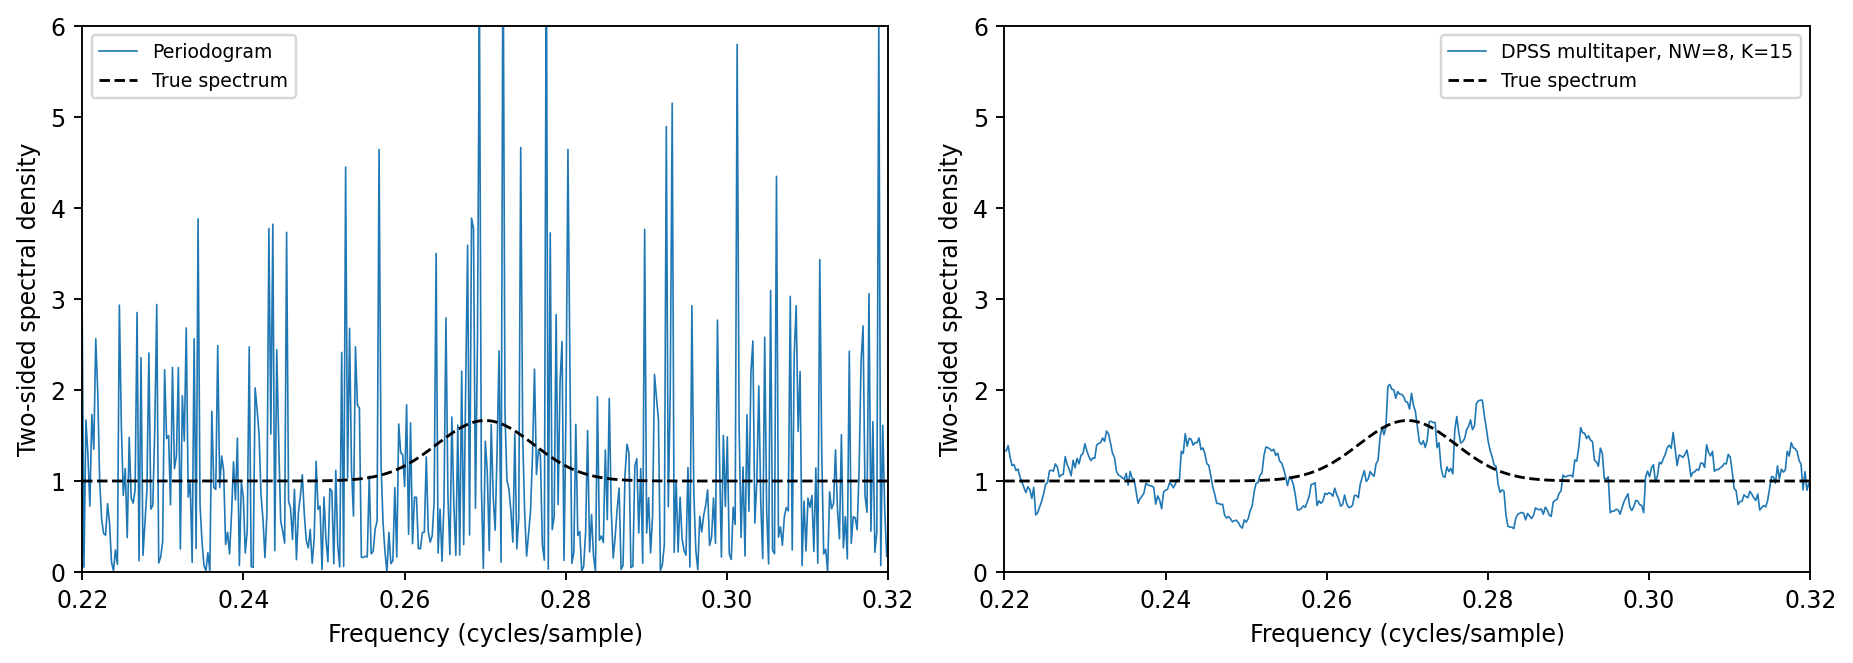
\includegraphics[width=0.98\linewidth]{png/problem2_faint_peak.png}
\caption{Weak spectral feature around $0.27$ on the same data. Both panels
use a common vertical range to make variance reduction visible.}
\label{fig:faint-peak}
\end{figure}
\vspace{1em}
\end{enumerate}
R functions like \texttt{spec.pgram} and \texttt{spec.mtm}, the latter being from the \texttt{multitaper} package, may be helpful. In both cases, you have multiple options for achieving this. You could design an ARMA process, but you may find it easier to design the \emph{spectrum} that makes the pathology obvious and then back out the ACF from it. \emph{You are welcome to use chatbots to solve hard integrals. But please be disciplined about restricting your use of them to just the hard integrals!}

\item A \emph{harmonic} of a fundamental frequency $f_0$ is an integer multiple $kf_0$ for $k\in\{2,3,4,\ldots\}$. Sometimes simple nonlinear transformations or other irregularities can cause your SDF estimator to also have peaks at these harmonics of ``true'' peaks. Let $n=2048$ or something like that, and consider the time series
\[
X_t=\tanh\bigl(\alpha\cos(2\pi f_0t+\phi)\bigr)+Z_t,
\]
where $Z_t$ is a white noise with variance $\sigma^2$, $f_0=0.05$, and $\phi\sim\operatorname{Unif}(0,2\pi)$. Simulate such an $X_t$. Does it look like it could be a stationary process? Look at a spectral density estimator for it as if it were, and play with values of $\alpha$ to make the harmonics more or less prominent. Then find another nonlinear function besides $\tanh$ to apply to your periodic function that also induces spurious harmonics in your estimator. Try to pick something interesting that gives you stationary-looking data!
\par\vspace{0.5em}\textbf{Sol.}\par

I use $n=2048$, $f_0=0.05$, independent Gaussian noise with
$\sigma=0.2$, and one uniform phase shared by the whole realization.
The code for the transformed signal is
\begin{lstlisting}[language=Python]
phase = rng.uniform(0, 2 * np.pi)
wave = np.cos(2 * np.pi * f0 * np.arange(n) + phase)
series = np.tanh(alpha * wave) + noise
\end{lstlisting}
With an independent i.i.d. noise process, this construction is strictly
stationary: shifting all times replaces the uniform phase by another
uniform phase modulo $2\pi$. A plot alone is not needed to establish this.

For small $\alpha$, $\tanh(\alpha\cos u)\approx\alpha\cos u$ and the
fundamental dominates. As $\alpha$ increases, saturation makes the waveform
closer to a square wave and odd harmonics appear. Half-period antisymmetry
excludes even harmonics in the noiseless signal. The DPSS estimates at the
third harmonic were approximately $0.0678$, $3.9716$, and $15.8890$ for
$\alpha=0.5,2,8$, respectively; the noise floor is about $0.04$.

As another nonlinearity I use half-wave rectification,
$g(u)=\max(u,0)$. Since
\[
g(\cos u)=\tfrac12\cos u+\tfrac12|\cos u|,
\]
it produces a nonzero constant, the fundamental, and even harmonics.
After subtracting the sample mean, the simulation shows the fundamental
near $0.05$ and peaks near $0.10$ and $0.20$. Random phase again ensures
stationarity, even though individual trajectories look periodic.

Strictly, these stationary random-phase processes have spectral atoms plus
the white-noise density. The plotted estimates smooth the atoms into peaks;
the periodic component does not have an ordinary Lebesgue spectral density.
Frequencies above Nyquist are aliased.
\begin{figure}[htbp]
\centering
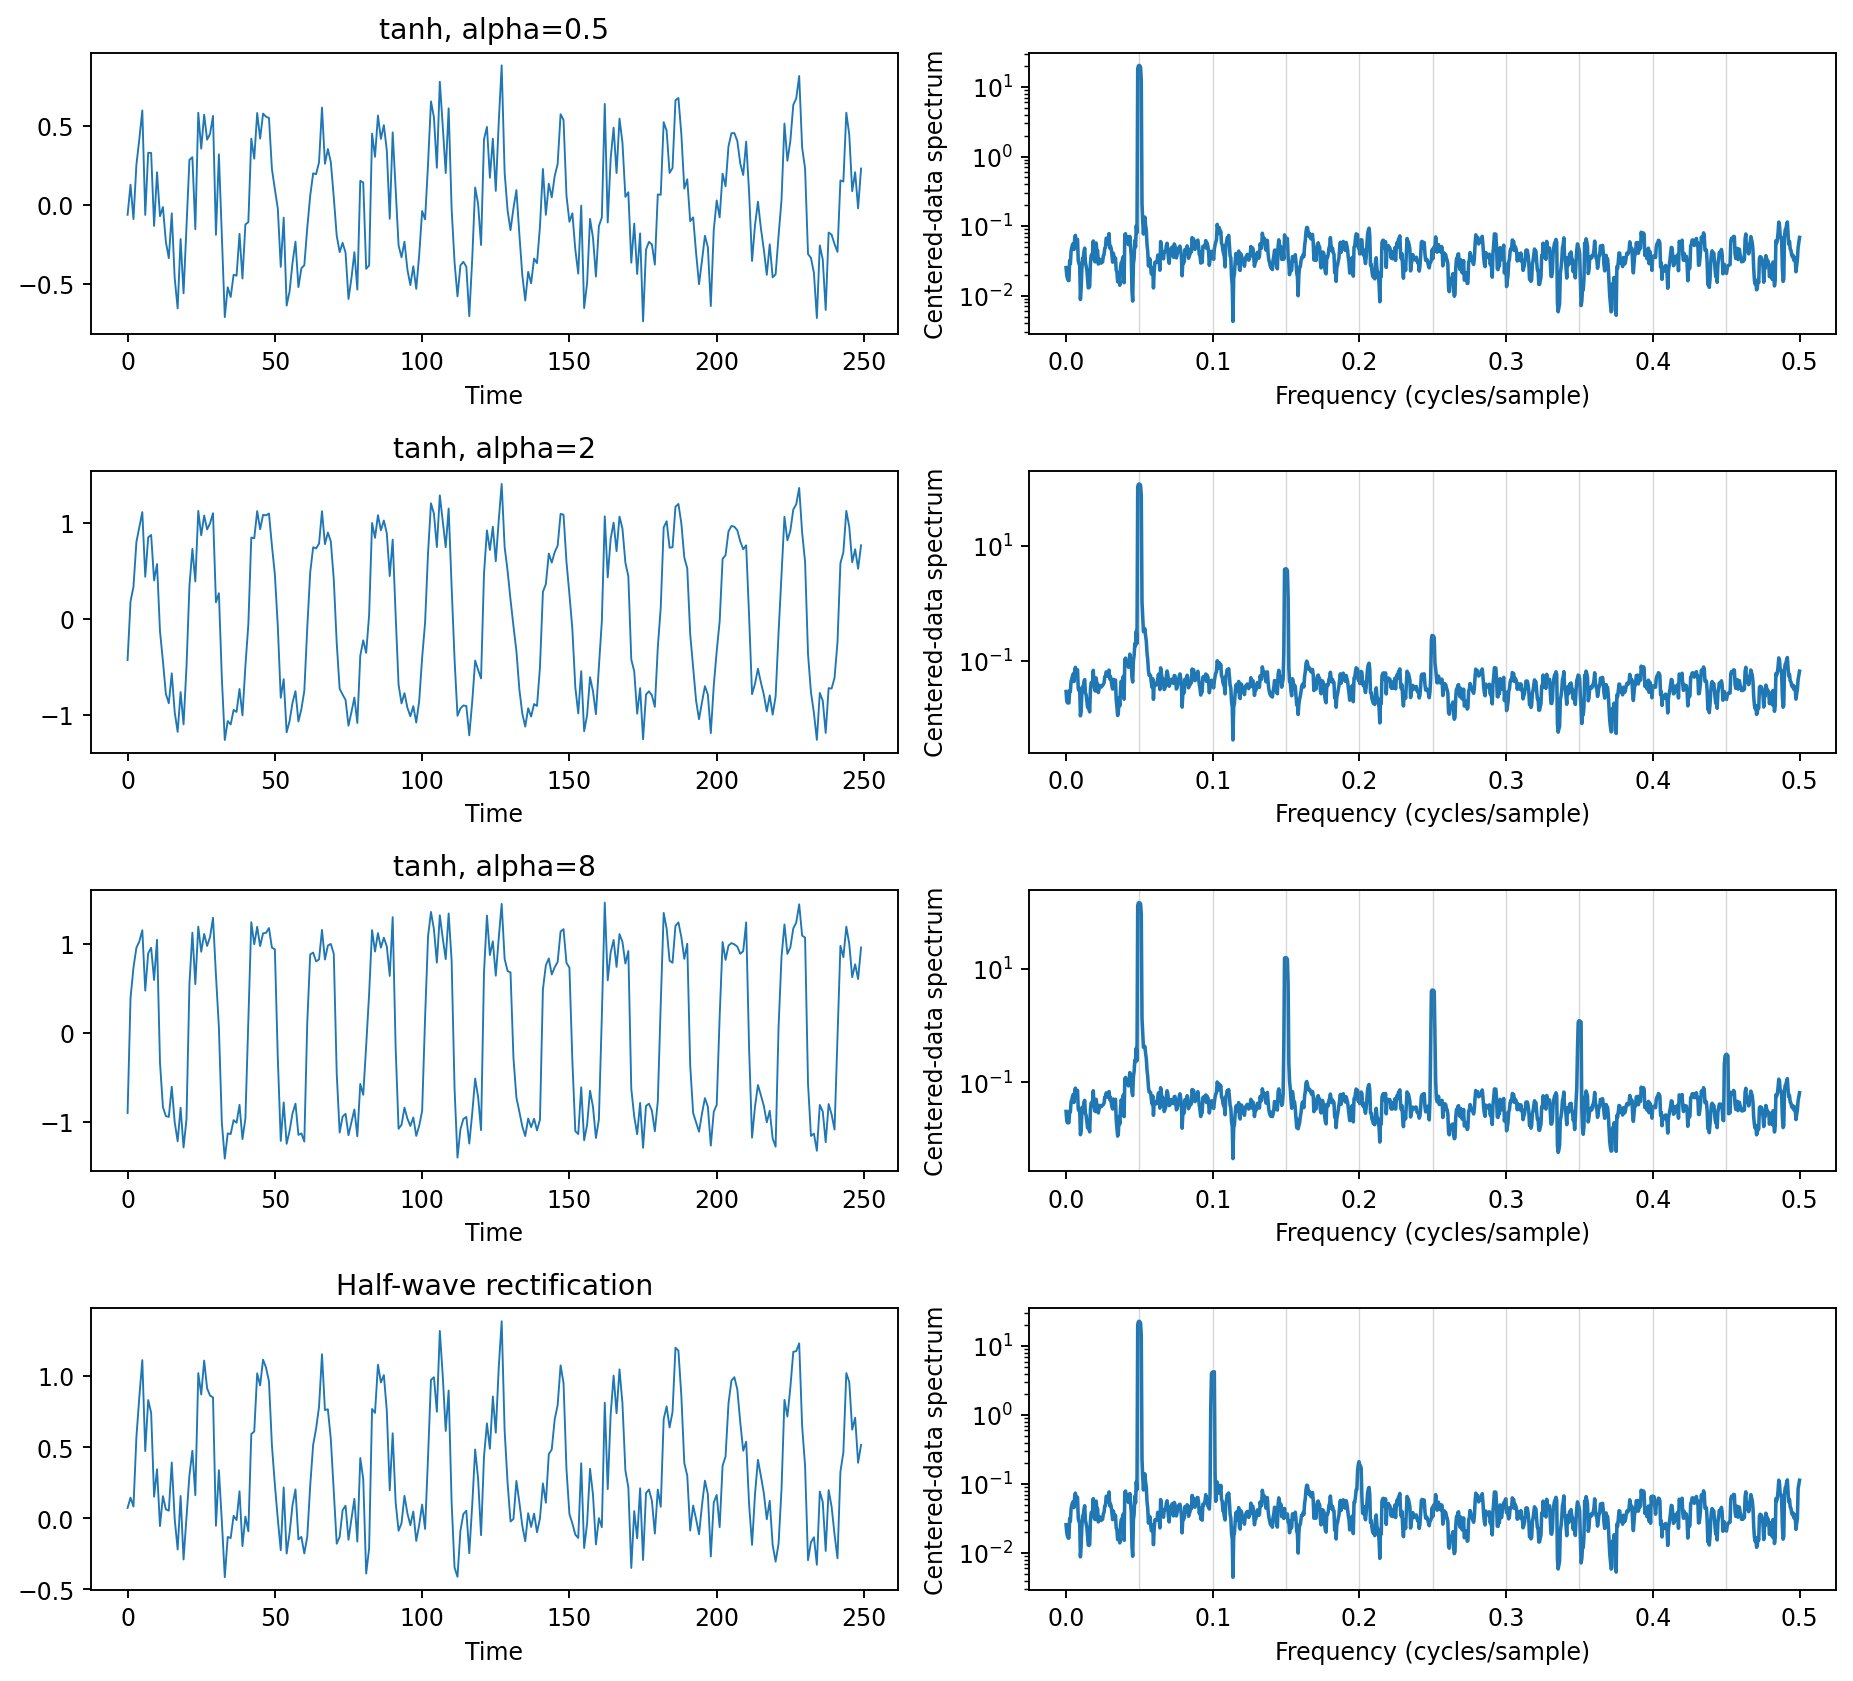
\includegraphics[width=0.95\linewidth]{png/problem2_harmonics.png}
\caption{Nonlinear random-phase signals and centered-data DPSS estimates
($NW=3$, five tapers). Vertical lines mark multiples of $f_0$.}
\label{fig:harmonics}
\end{figure}
\vspace{1em}

\item Pull the tide gauge data from Canvas. Pick a segment of moderate length (at least a few thousand points) with no gaps, and compute several spectral density estimators: a periodogram, a sine multitaper, a DPSS multitaper, and whatever else your heart desires. Inspect each of them and try to answer: how many of these peaks are real, and how many are harmonics? How would you model this spectral density? You might consider taking a look at a list of lunar frequencies, which you can find on, e.g., Wikipedia. You don't have to include an answer to this part of the question, but try to ponder: how might you distinguish that non-linear mean from structure in a stationary covariance function?
\par\vspace{0.5em}\textbf{Sol.}\par

I use the supplied \texttt{tidegauge.csv}, which has date fields
\texttt{year, month, day, hour} and observations in \texttt{actual}.
All 119,266 rows have finite observations and consecutive hourly timestamps.
I select the first 8192 observations, from October 1, 1980 at 13:00 to
September 7, 1981 at 20:00, without interpolation. The frequency grid spacing
is $24/8192=0.00292969$ cycles per day; the DPSS half-bandwidth with $NW=4$
is $0.01171875$ cycles per day.

The code compares the ordinary periodogram, seven sine tapers, and seven
unit-norm DPSS tapers. It subtracts the segment mean before computing spectra:
\begin{lstlisting}[language=Python]
time = pd.to_datetime(table[["year", "month", "day", "hour"]])
values = table["actual"].to_numpy()
series = values[:8192] - values[:8192].mean()
f, raw = periodogram(series)
f, sine = multitaper_spectrum(series, sine_tapers(8192, 7))
f, mt = multitaper_spectrum(
    series, dpss(8192, NW=4, Kmax=7, norm=2)
)
\end{lstlisting}
For conversion from cycles per hourly observation to cycles per day I
multiply frequency by 24 and divide density by 24, preserving integrated
spectral power. The periodogram resolves sharper lines but fluctuates more;
both multitaper estimates give smoother peaks with wider tops.

There are at least five prominent astronomical peak groups, around $0.93$,
$1.00$, $1.90$, $1.93$, and $2.00$ cycles per day. The strongest diurnal and
semidiurnal components are consistent with the standard constituent
frequencies below. The raw-grid peaks are approximate locations, not
new estimates precise to all the quoted reference digits.
\begin{center}
\begin{tabular}{lrr}
\hline
Constituent & Reference frequency (cycles/day) & Nearby raw peak \\
\hline
$O_1$ & $0.92954$ & $0.92871$ \\
$K_1$ & $1.00274$ & $1.00195$ \\
$N_2$ & $1.89598$ & $1.89551$ \\
$M_2$ & $1.93227$ & $1.93359$ \\
$S_2$ & $2.00000$ & $2.00098$ \\
\hline
\end{tabular}
\end{center}
The reference speeds and constituent descriptions follow the
\href{https://tidesandcurrents.noaa.gov/harcon.html?id=8721120}{NOAA harmonic-constituent table};
only its universal frequencies are used, not another station's amplitudes.
The $P_1/K_1$ and $S_2/K_2$ separations are smaller than the multitaper
smoothing width, so these should be treated as unresolved groups in that
plot. Smaller lunar constituents, such as $Q_1$, can also contribute.

A peak near twice a diurnal frequency need not be its harmonic: $M_2$ and
$S_2$ are distinct astronomical forcing constituents. Conversely, weaker
features near $3.8643$ and $3.9229$ cycles per day are compatible with the
\emph{overtide} $M_4$ at $2f_{M_2}=3.86455$ and the compound constituent $MS_4$
at $f_{M_2}+f_{S_2}=3.93227$, within the smoothing resolution. Other weak
features occur near $2.8975$, $3.0059$, and $4.0049$. These are candidates
for higher or compound harmonics, but the plot alone cannot assign every
one uniquely. They can be physical nonlinear tidal signals rather than
estimation artifacts. Thus counting every local maximum as an independent
oscillation would overstate what the data resolve; there is no unambiguous
single count of ``real'' versus ``spurious'' peaks from these estimates alone.

A useful model is a deterministic harmonic mean plus a stochastic residual:
\[
X_t=\mu+\beta t+\sum_j\{a_j\cos(2\pi f_jt)+b_j\sin(2\pi f_jt)\}
+\varepsilon_t,
\]
where $t$ is measured in days. I fit an intercept, a linear trend, eight
principal astronomical constituents ($Q_1,O_1,P_1,K_1,N_2,M_2,S_2,K_2$),
and three overtide/compound candidates ($M_4,MS_4,M_6$) by least squares.
This descriptive fit explains $91.58\%$ of the centered segment variance;
its residual mean square is $0.002695$ in squared supplied-data units.
The dominant spectral peaks fall substantially after regression, although
some narrow components and low-frequency residual variation remain.
A smooth colored spectrum or an ARMA model for $\varepsilon_t$, with any
remaining reproducible lines explicitly modelled, would be a reasonable
next step.

The variance explained is in-sample, not a prediction score. To distinguish
a nonlinear mean from stationary covariance structure, I would check phase
coherence relative to astronomical forcing across disjoint windows and
validate predictions and residuals on held-out periods. A stationary
random-phase process can have the same spectral lines, so second-order
spectral information alone cannot settle this distinction.
\begin{figure}[htbp]
\centering
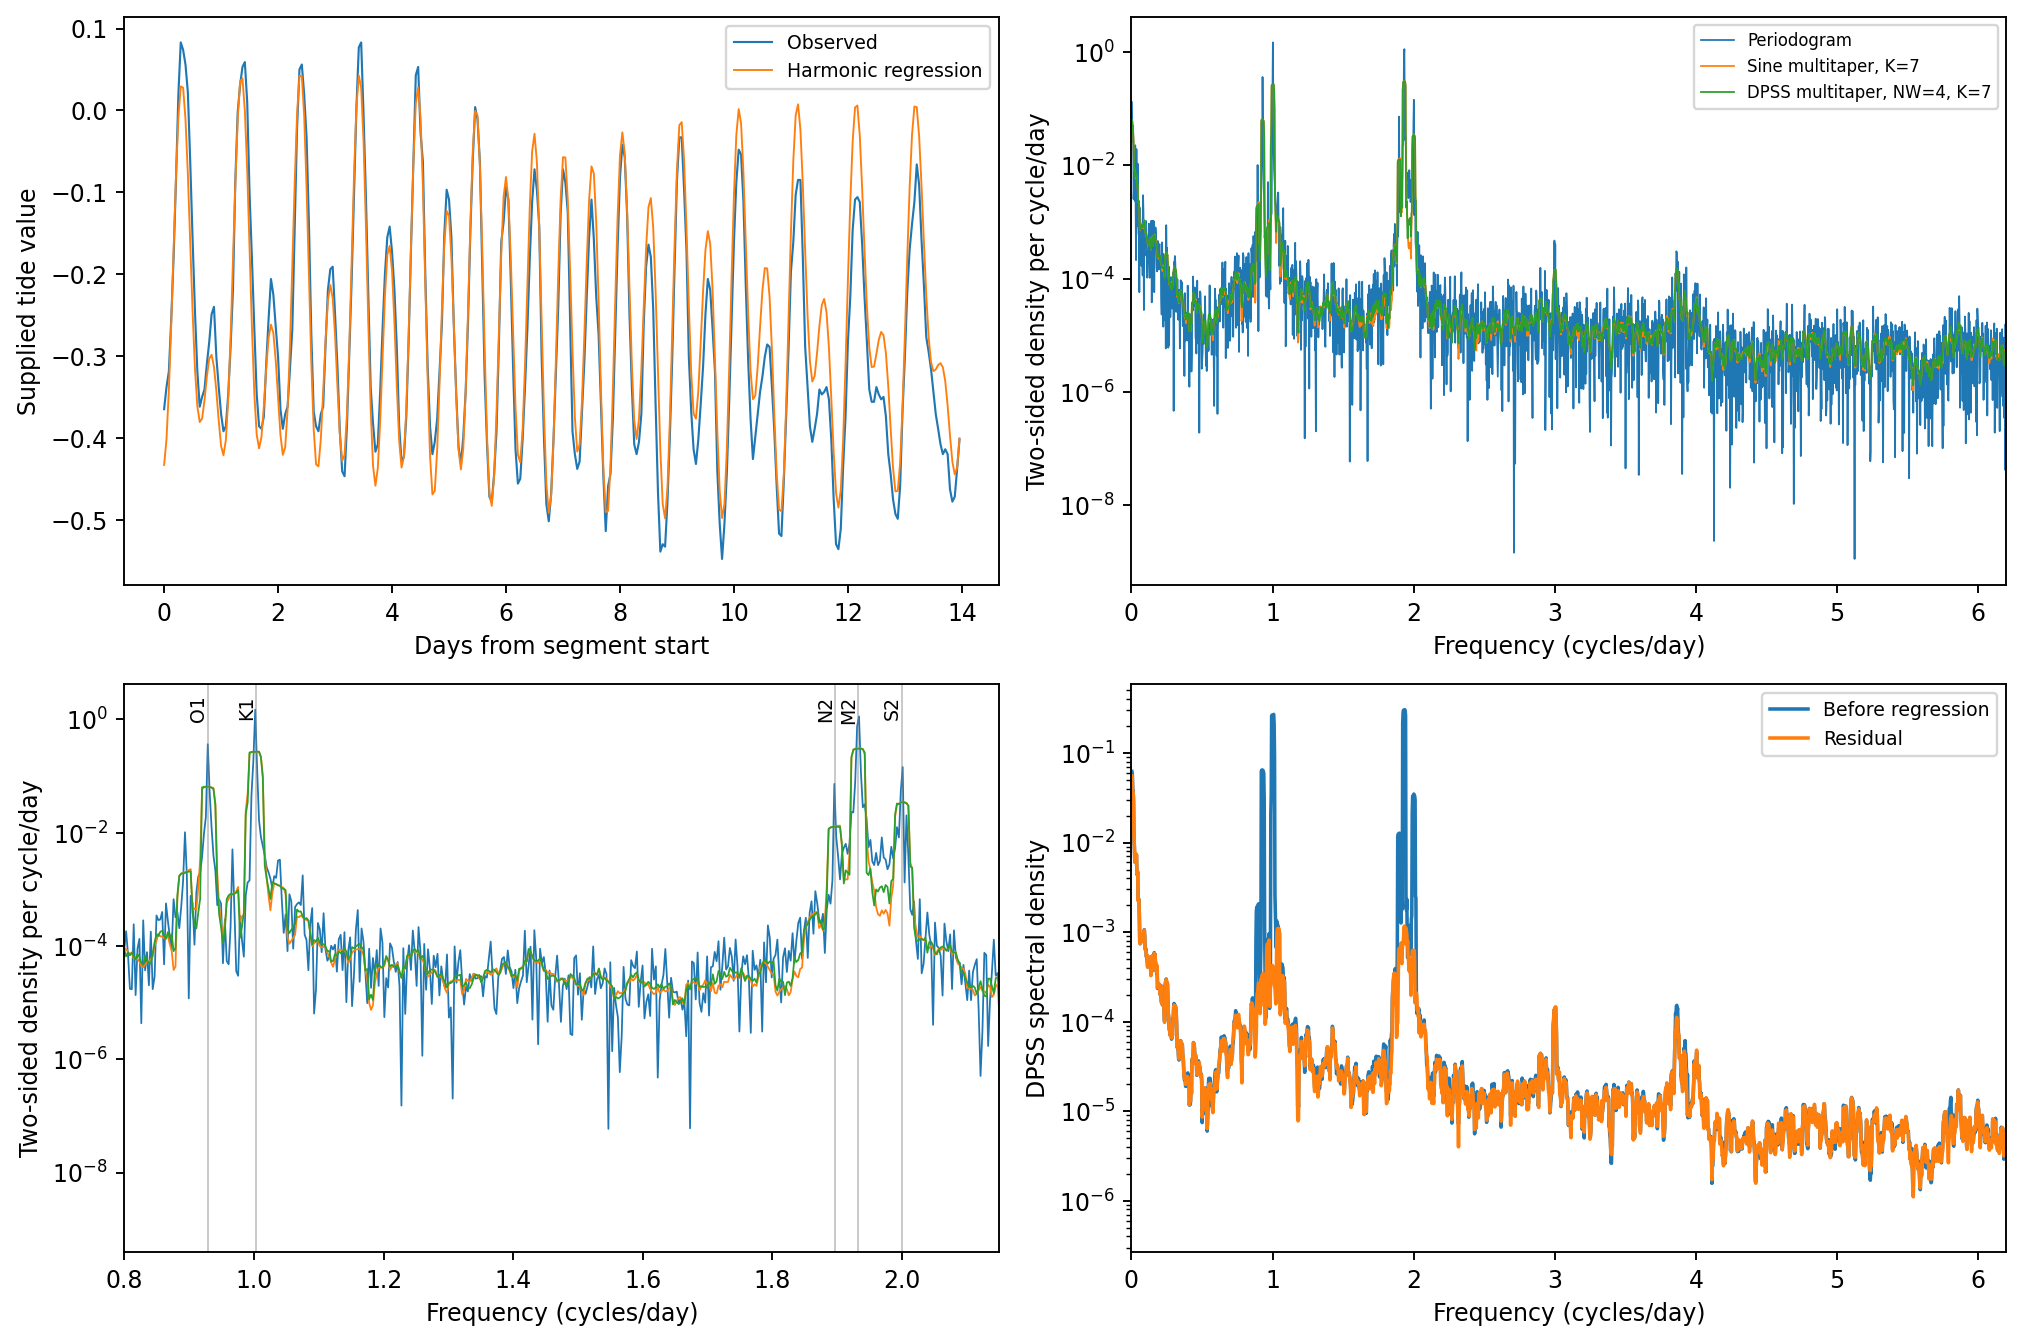
\includegraphics[width=0.99\linewidth]{png/problem2_tide.png}
\caption{Observed hourly tide data, spectral estimates, and harmonic-regression
residuals for the selected gap-free 8192-point segment.}
\label{fig:tide-analysis}
\end{figure}
\vspace{1em}
\end{enumerate}

\FloatBarrier
\subsection*{Problem 3}
Write code to implement the \emph{Whittle likelihood} described in class. In particular, please write a function that takes two arguments: the (potentially weighted) DFT of your data, and SDF parameters.
\begin{enumerate}[label=\arabic*.,leftmargin=*]
\item Pull up the NAO data and take the first 1024 measurements. Look at an exploratory estimator for the spectrum (perhaps a multitaper\ldots) and find a functional form you like for the spectrum. This should be something involving parameters, like $S_\theta(\omega)=\theta_0e^{-\theta_1|\omega|}$ or something. Discuss your choices.
\par\vspace{0.5em}\textbf{Sol.}\par

I use the first 1024 daily measurements without gaps and subtract their
sample mean, $\bar X=-0.34727$. As in HW2, the file is named
\texttt{nao.csv}, but its supplied value column is labelled
\texttt{aao\_index\_cdas}; I analyze the supplied values without relabelling
them as a different downloaded index.

The periodogram and a seven-taper DPSS estimate ($NW=4$) show strong
low-frequency power with an overall declining envelope and a small
high-frequency floor. I choose the three-parameter family
\[
S_\theta(f)=a e^{-b|f|}+c,\qquad
-\tfrac12\leq f\leq\tfrac12,\qquad a,b,c>0.
\]
This is a simple positive even spectrum: $a$ controls the excess amplitude,
$b$ controls its decay, and $c$ represents a white-noise floor. It captures
the broad shape without treating every noisy periodogram spike as a
separate physical component. It is a deliberately parsimonious working
model, not a claim that the true spectrum must be monotone.
\begin{figure}[htbp]
\centering
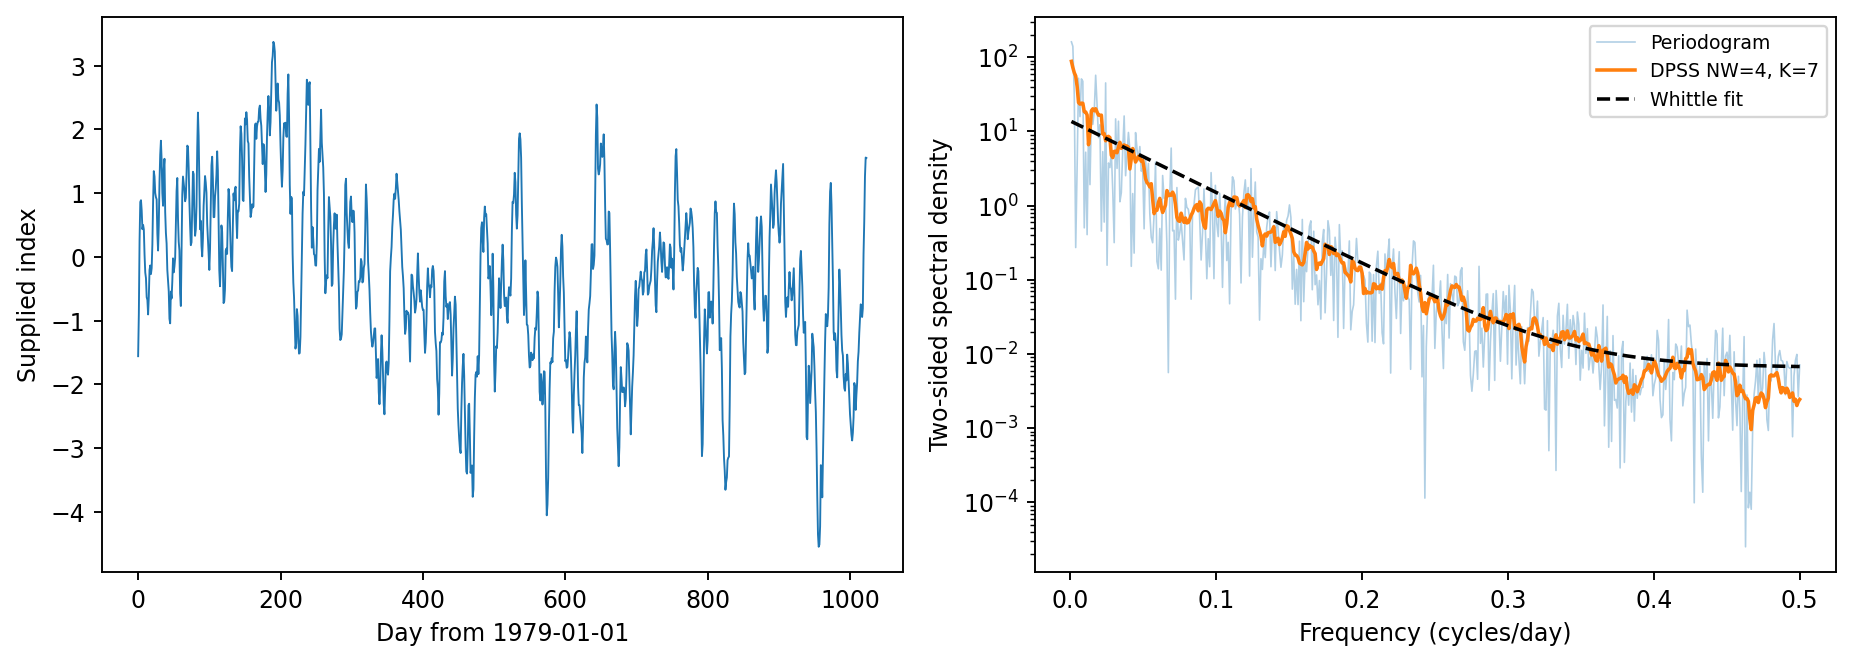
\includegraphics[width=0.98\linewidth]{png/problem3_whittle_fit.png}
\caption{First 1024 supplied daily measurements and the fitted spectral
shape, using two-sided density in cycles per day.}
\label{fig:whittle-fit}
\end{figure}
\vspace{1em}

\item By specifying your Whittle likelihood and handing that function to an optimizer (be careful about bound constraints for valid parameters!), fit that functional form to the data.
\par\vspace{0.5em}\textbf{Sol.}\par

I compute $d_k=n^{-1/2}\sum_{t=0}^{n-1}(X_t-\bar X)e^{-2\pi ikt/n}$
and $I_k=|d_k|^2$. For real data I use only the positive frequencies,
with the real-valued Nyquist coefficient given half weight:
\[
Q(\theta)=\sum_{k=1}^{n/2-1}
\left[\log S_\theta(k/n)+\frac{I_k}{S_\theta(k/n)}\right]
+\frac12\left[\log S_\theta(1/2)+\frac{I_{n/2}}{S_\theta(1/2)}\right].
\]
The zero frequency is excluded after estimating the mean. The DFT time
origin differs from Problem 1 only by a unit-modulus phase and therefore
does not change the periodogram. The two-sided spectrum is not doubled
when only positive frequencies are used in this likelihood.
\begin{lstlisting}[language=Python]
dft = np.fft.fft(series) / np.sqrt(len(series))
parameters, result = fit_spectrum(dft)
\end{lstlisting}
I optimize the log parameters with bounded L-BFGS-B and four initial decay
values. All fitted parameters are positive; the selected optimizer reports
convergence. The fitted spectrum is
\[
\widehat S(f)=13.89572e^{-22.24673|f|}+0.00658014,
\]
with objective $Q=-638.94618$, up to the omitted parameter-independent
likelihood constants. This formula uses cycles per day; coefficients cannot
be transferred unchanged to an angular-frequency density.
For weighted DFT inputs the same function is a Whittle-type approximation;
tapering smooths the expected periodogram and correlates nearby coefficients.
The fit reported here uses the untapered DFT to keep this approximation clear.
\vspace{1em}

\item[$3^*$.] Using a numerical integrator or a chatbot or however you please, get from the spectral density to obtaining the corresponding ACF values $\{\gamma(0),\ldots,\gamma(n-1)\}$. Now take your fitted model SARIMA model from last week and evaluate the true likelihood, involving the covariance matrix and stuff, for each fitted model. Which of the two models has a better likelihood? Try and investigate what you think is going on and why one or the other was better.
\par\vspace{0.5em}\textbf{Sol.}\par

Fourier inversion gives an analytic autocovariance. For integer $h$,
\begin{align*}
\gamma_\theta(h)
&=2a\int_0^{1/2}e^{-bf}\cos(2\pi hf)\,df+c\,1_{\{h=0\}}\\
&=\frac{2ab\{1-(-1)^he^{-b/2}\}}{b^2+(2\pi h)^2}
+c\,1_{\{h=0\}}.
\end{align*}
Numerical quadrature at lags $0,1,10,100,1023$ agreed with this expression
to better than $10^{-7}$. Let $\Gamma_{ij}=\gamma_\theta(i-j)$.
The exact Gaussian log likelihood for centered observations is
\[
\ell=-\frac12\{n\log(2\pi)+\log\det\Gamma+x^\top\Gamma^{-1}x\}.
\]
The code uses a Cholesky factor and triangular solves rather than an explicit
inverse. For the 1024-point vector, the fitted stationary model gives
$\ell=-228.49829$, treating the sample-mean estimate as a fixed plug-in value.

The previous HW2 fit was
\[
(1-.6642B-.3518B^2+.2324B^3-.0837B^4)(1-B^{365})X_t
=(1+1.1556B+.3247B^2)Z_t,
\]
with innovation variance $0.1956$. This SARIMA model has a seasonal unit
root, so it has no stationary covariance matrix for the raw levels.
Comparing a raw-data stationary likelihood against a likelihood of
differenced data would use different observations and be misleading.
Instead I evaluate both fitted models on the same 659-dimensional vector
$Y_t=X_{t+365}-X_t$. For the stationary spectral model,
\[
\gamma_Y(h)=2\gamma(h)-\gamma(h+365)-\gamma(h-365).
\]
For the SARIMA model, $Y$ is the stationary ARMA$(4,2)$ process above.
Using the rounded coefficients reported in HW2, the exact marginal Gaussian
log likelihoods of this common data vector are
\[
\ell_{\mathrm{spectral}}(Y)=-344.26496,
\qquad
\ell_{\mathrm{SARIMA}}(Y)=-366.31558.
\]
Thus the spectral model has the larger likelihood by $22.05062$ on this
common differenced sample. These are marginal likelihoods of the
\emph{differences}, not unconditional likelihoods for the original levels.
A conditional-level comparison would additionally require specifying how
the SARIMA innovations relate to the initial seasonal levels.

This result is consistent with the weak annual dependence noted in HW2:
forcing annual integration may be a poor description of this segment.
The comparison is descriptive, not an out-of-sample test: the old coefficients
were fitted on the larger record, whereas the spectral model was fitted to
these first 1024 observations, and the models have different complexity.
Nor is the new model perfect. Its variance is $1.25580$, compared with the
centered sample variance $1.87984$, and its ACF misses the slower empirical
component. Whittle diagonalization, finite-window effects and spectral
misspecification can all contribute to this discrepancy.
\begin{figure}[htbp]
\centering
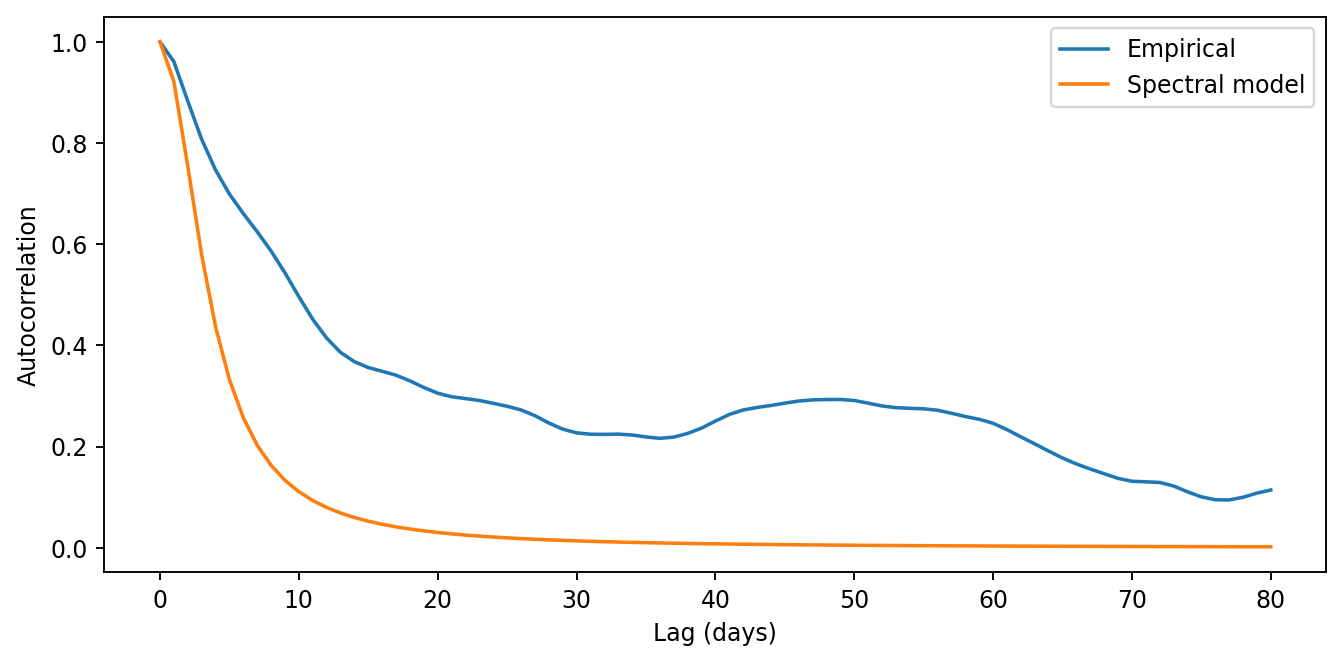
\includegraphics[width=0.85\linewidth]{png/problem3_acf.png}
\caption{Empirical and fitted autocorrelation functions. The simple fitted
spectrum does not reproduce all long-lag dependence.}
\label{fig:fitted-acf}
\end{figure}
\vspace{1em}
\end{enumerate}

\FloatBarrier
\clearpage
\appendix
\section{Python code}
The following scripts reproduce the simulations, estimates, and figures.
Data are stored in \texttt{data/}; figures are written to \texttt{png/}.
The supplied tide data are included in \texttt{data/tidegauge.csv}.
The scripts contain no comments. All spectral estimates use the two-sided
density convention even when only positive frequencies are displayed.

\subsection{Problem 1}
\lstinputlisting[language=Python,basicstyle=\ttfamily\scriptsize]{code/problem1.py}
\clearpage
\subsection{Problem 2}
\lstinputlisting[language=Python,basicstyle=\ttfamily\scriptsize]{code/problem2.py}
\clearpage
\subsection{Problem 3}
\lstinputlisting[language=Python,basicstyle=\ttfamily\scriptsize]{code/problem3.py}

\end{document}
